\begin{figure}[t]
\centering
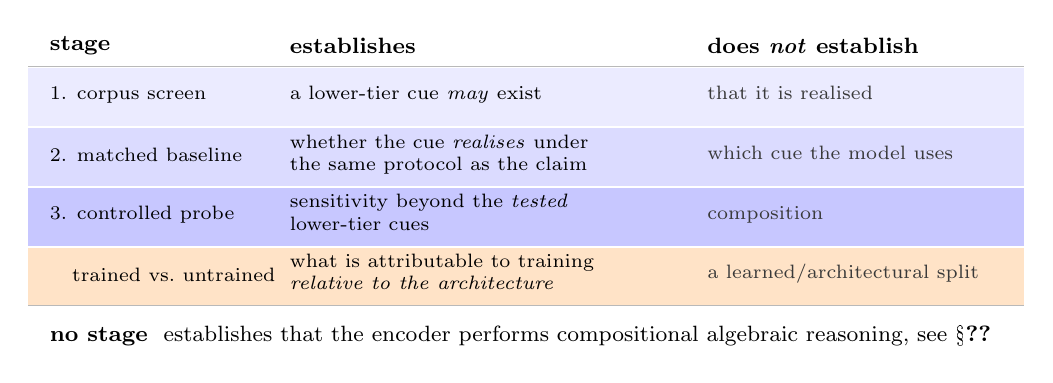
\begin{tikzpicture}[font=\scriptsize, node distance=0pt]

\def\rowh{0.76}
\def\colA{0}      % stage
\def\colB{3.05}   % establishes
\def\colC{8.35}   % does NOT establish

% header
\node[anchor=west, font=\footnotesize\bfseries] at (\colA, 0.62) {stage};
\node[anchor=west, font=\footnotesize\bfseries] at (\colB, 0.62) {establishes};
\node[anchor=west, font=\footnotesize\bfseries] at (\colC, 0.62) {does \emph{not} establish};
\draw[gray!55] (-0.15, 0.36) -- (12.5, 0.36);

\foreach \i/\stage/\yes/\no/\col in {
  0/{1. corpus screen}/{a lower-tier cue \emph{may} exist}/{that it is realised}/blue!8,
  1/{2. matched baseline}/{whether the cue \emph{realises} under \\ the same protocol as the claim}/{which cue the model uses}/blue!14,
  2/{3. controlled probe}/{sensitivity beyond the \emph{tested} \\ lower-tier cues}/{composition}/blue!22,
  3/{\ \ \ trained vs.\ untrained}/{what is attributable to training \\ \emph{relative to the architecture}}/{a learned/architectural split}/orange!22}
{
  \pgfmathsetmacro{\yy}{-\i*\rowh}
  \fill[\col] (-0.15, \yy+0.34) rectangle (12.5, \yy-0.40);
  \node[anchor=west, align=left] at (\colA, \yy) {\stage};
  \node[anchor=west, align=left] at (\colB, \yy) {\begin{tabular}{@{}l@{}}\yes\end{tabular}};
  \node[anchor=west, align=left, gray!45!black] at (\colC, \yy) {\begin{tabular}{@{}l@{}}\no\end{tabular}};
}

\draw[gray!55] (-0.15, -3*\rowh-0.40) -- (12.5, -3*\rowh-0.40);
\node[anchor=west, align=left, font=\footnotesize] at (\colA, -3*\rowh-0.78)
  {\textbf{no stage}\ \ establishes that the encoder performs compositional algebraic reasoning,
   see \S\ref{sec:tier3}};

\end{tikzpicture}
\caption{\textbf{What each stage licenses.} The tools form a pipeline, and conflating its stages is
what produces overclaims. A claim is worth exactly the highest floor it clears: the screen is a cheap
pre-training diagnostic that says where to look, only the matched baseline licenses a statement about
a \emph{benchmark}, and only the controlled probe licenses one about a \emph{model}. The two
non-learned families answer different questions and are reported separately throughout: a
\textbf{bag} is a structure-free lower-tier floor, an \textbf{untrained encoder} is an
architecture-sensitive non-learned floor that already computes over structure.}
\label{fig:pipeline}
\end{figure}
